\chapter{Hardware implementeringen og operativ system}\label{kap:hardware}

I dette kapitel vil den komplette software og hardware løsning blive gennemgået som gør det muligt at udfører den digitale behandling af lydsignalet.
\husk{JJ}{Kort beskrivelse af de mellemliggende trin}
Til sidst vil der være en gennemgang af de nærliggende forbedringer og optimeringer.


\begin{enumerate}
	\item Overblik af OS, lagdelt model
	\item Beskrivelse af Hardware lag - beskrivelse af de forskellige setups og hvorfor - fordele og ulæmper.
	\begin{enumerate}
		\item Initalisering af systemet som helhed - fastsættelse af beregningspunkter.
		\item Fastsættelse af clockfrekvens
		\item ADC (simon)
		\item LCD Driver (søren)
		\item UART (Søren)
		\item DAC / SPI
	\end{enumerate}
	\item håndtering af indgående lyssignal i de forskellige modes
	\item FPU math
	\item Schedulering af taskt - task model 
	\item Beskrivelse af de enkelte tasks
	\item Shell (ANSI / VT100) (Søren ?) 
	\item Quealizer profile model
	\item Debugging og task time profiling
	
\end{enumerate}

\section{Det vigtigste er lyden}
Den absolut primære funktion af equalizeren   


\husk{JJ}{sektion der beskriver indledende hvordan tilgangen til design af OS har været med baggrund i krav om sampling og gengivelse i realtime}

\section{Operativ systemet}

\begin{figure}[h!]
	\centering
	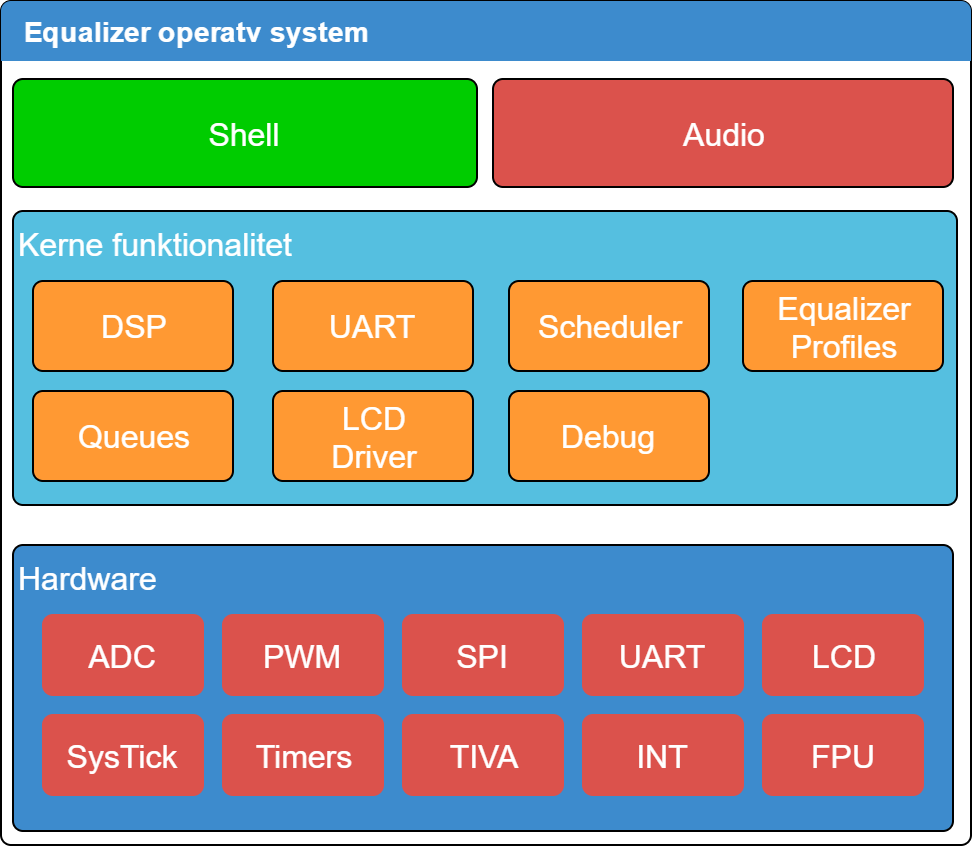
\includegraphics[width=.8\textwidth]{billeder/eq_os.png}
	\caption{Arkitektur af equalizerens operativ system.}
	\label{fig:eq_os}
\end{figure}
\FloatBlock


\section{Schedulering}




\section{Hardware lag}



\subsection{ADC}
En analog til digital konverter kan anvendes til at konvertere et sammenhængende analogt spændingssignal til et diskret digitalt nummer. TMC4C123GH6PM microcontrolleren har to identiske 12 bit A/D konvertere indbygget - ADC0 og ADC1. Det konverterede signal, kan derefter behandles vha. digitale signalbehandlingsmetoder. 
Da der ønskes at opbygge en stereostyret equalizer, bruges begge A/D konvertere. Konfigurationen er derfor ens på hhv. ADC0 og ADC1. Begge A/D konvertere kører uafhængigt af hinanden. Afhængig af hvilken Sample frequencer der er valgt, gemmes
resultatet af A/D konverteringen i et FIFO register (first in - first out). Da der kun er brug for én sample ad gangen, vælges ud fra databladet at konfigurere A/D konverterne med Sample sequencer 3, og derved gemmes resultatet af konverteringen også i ADCSSFIFO3 registeret for hhv. ADC0 og ADC1.
Da det ikke er alle porte, der kan anvendes på microcontrolleren til A/D konvertering, er pin PB5 valgt til at styre venstre kanal, og pin PE4 er valgt til at styre højre kanal. Herudover kan den også køre i mono, frem for stereo - denne er konfigureret på pin PE5. Der ønskes en samplingsfrekvens på $44,1\si\kilo\hertz$ for at undgå aliasing. Denne samplingsfrekvens er bestemt ud fra Nyquist frekvensen. For at få denne samplingsfrekvens korrekt, skal microcontrollerens CPU frekvens sættes til $80\si\mega\hertz$. Der bruges et PWM signal, som er interruptstyret. Dette signal skal køre et bestemt antal cycles.

\begin {equation}
\text{Cycles} = \frac{\text{CPU frekvens}}{\text{Sample frekvens}} => \frac{80\cdot 10^6\si\hertz}{44100\si\hertz} = 1814 \text{cycles}
\end {equation}

Hver gang PWM'en har kørt i det beregnede antal cycles, bliver et interrupt initialiseret, og samplingen starter samt gemmer værdien. Ved næste interrupt, starter processen for A/D konverteringen igen.
Da A/D konverterne er opløst i 12 bit, og den maksimale spænding der bliver registreret er $3,3\si\volt$ - vil maksimalværdien for konverteringen være $4096$. 

\section{Equalizer modul og profiler}

\section{Shell}

\section{Debugging, process timing og mulige udfordringer}

\section{Pin mapping}

\husk{JJ}{Oversæt excel ark til \LaTeX}
\husk{JJ}{Dettte skema skal overflyttes som bilag}

\section{Udvidelser}

\begin{enumerate}
	\item I2C intraface
	\item Flash lager
	\item Flere shell commmandoer
\end{enumerate}
